\chapter{Reflection}

This chapter illustrates various aspects reside in the management of the project, including a revision of the original workplan, a description of the working methodology, resource management details and contingency measures. A personal reflection to the project is also presented. 

\section{Project Management}
% Covering the tasks as a part of your work plan and progress as well as how time and resources are managed.

\subsection{Revision of Workplan}
% Revision of workplan.
Figure \ref{fig:Gantt_old} shows the proposed workplan of the project designed at the beginning stage. Generally speaking, the progress of the project has been satisfying, as all the phases involving literature review and systematic learning have been completed on time. One task was shelved and left behind schedule, however, namely the delivery of an ontology matching framework, which was supposed to come along with the interim report. There are two primary contributing factors to the making of this decision. Firstly, the workload in studying existing ontology matching techniques was underestimated, making the expectation of designing the framework simultaneously with the learning process unrealistic. Secondly, time allocation was inevitably tilted to the investigation of instance matching strategies, as they are inseparable from the general ontology matching framework. This was considered better for the selection of suitable framework components after some investigation into ontology matching, and was hence given higher priority.
\\\\
In order to reflect the above changes, a revised workplan was designed after reaching the Interim Report milestone, and is presented in figure \ref{fig:Gantt_new}. The new workplan demonstrates how the previous stages had been completed, as well as how the second half of the project was designed to progress. Due to the effect of autumn semester exam preparation, implementation tasks before the exams were only preliminary, while the major development tasks were put in the winter vacation. Since coding and debugging can take a large amount of time, this decision was proved to be sensible. The adjustment of ontology matching algorithm was redesigned to be side by side with testing and evaluation, with the validation of design carried all along the way. This was to target the unexpected obstacles and potential risks such as increased academic workload during the spring semester, in which case the adjustment phase can shrink to buffer the impact on the overall workplan. This was proved to be extremely effective, as unforeseen difficulties within the project implementation stage could not have been countered without the degree of flexibility in the timeframe. The workload of writing the final dissertation was spread over a longer timespan, as it was discovered that writing usually takes longer than expected. Although time was still scheduled very tightly at the final stage of the project because of the difficulty of implementation, everything was able to be delivered on time thanks to following the revised workplan.

\begin{figure}[ht]
\begin{subfigure}[ht]{0.5\textwidth}
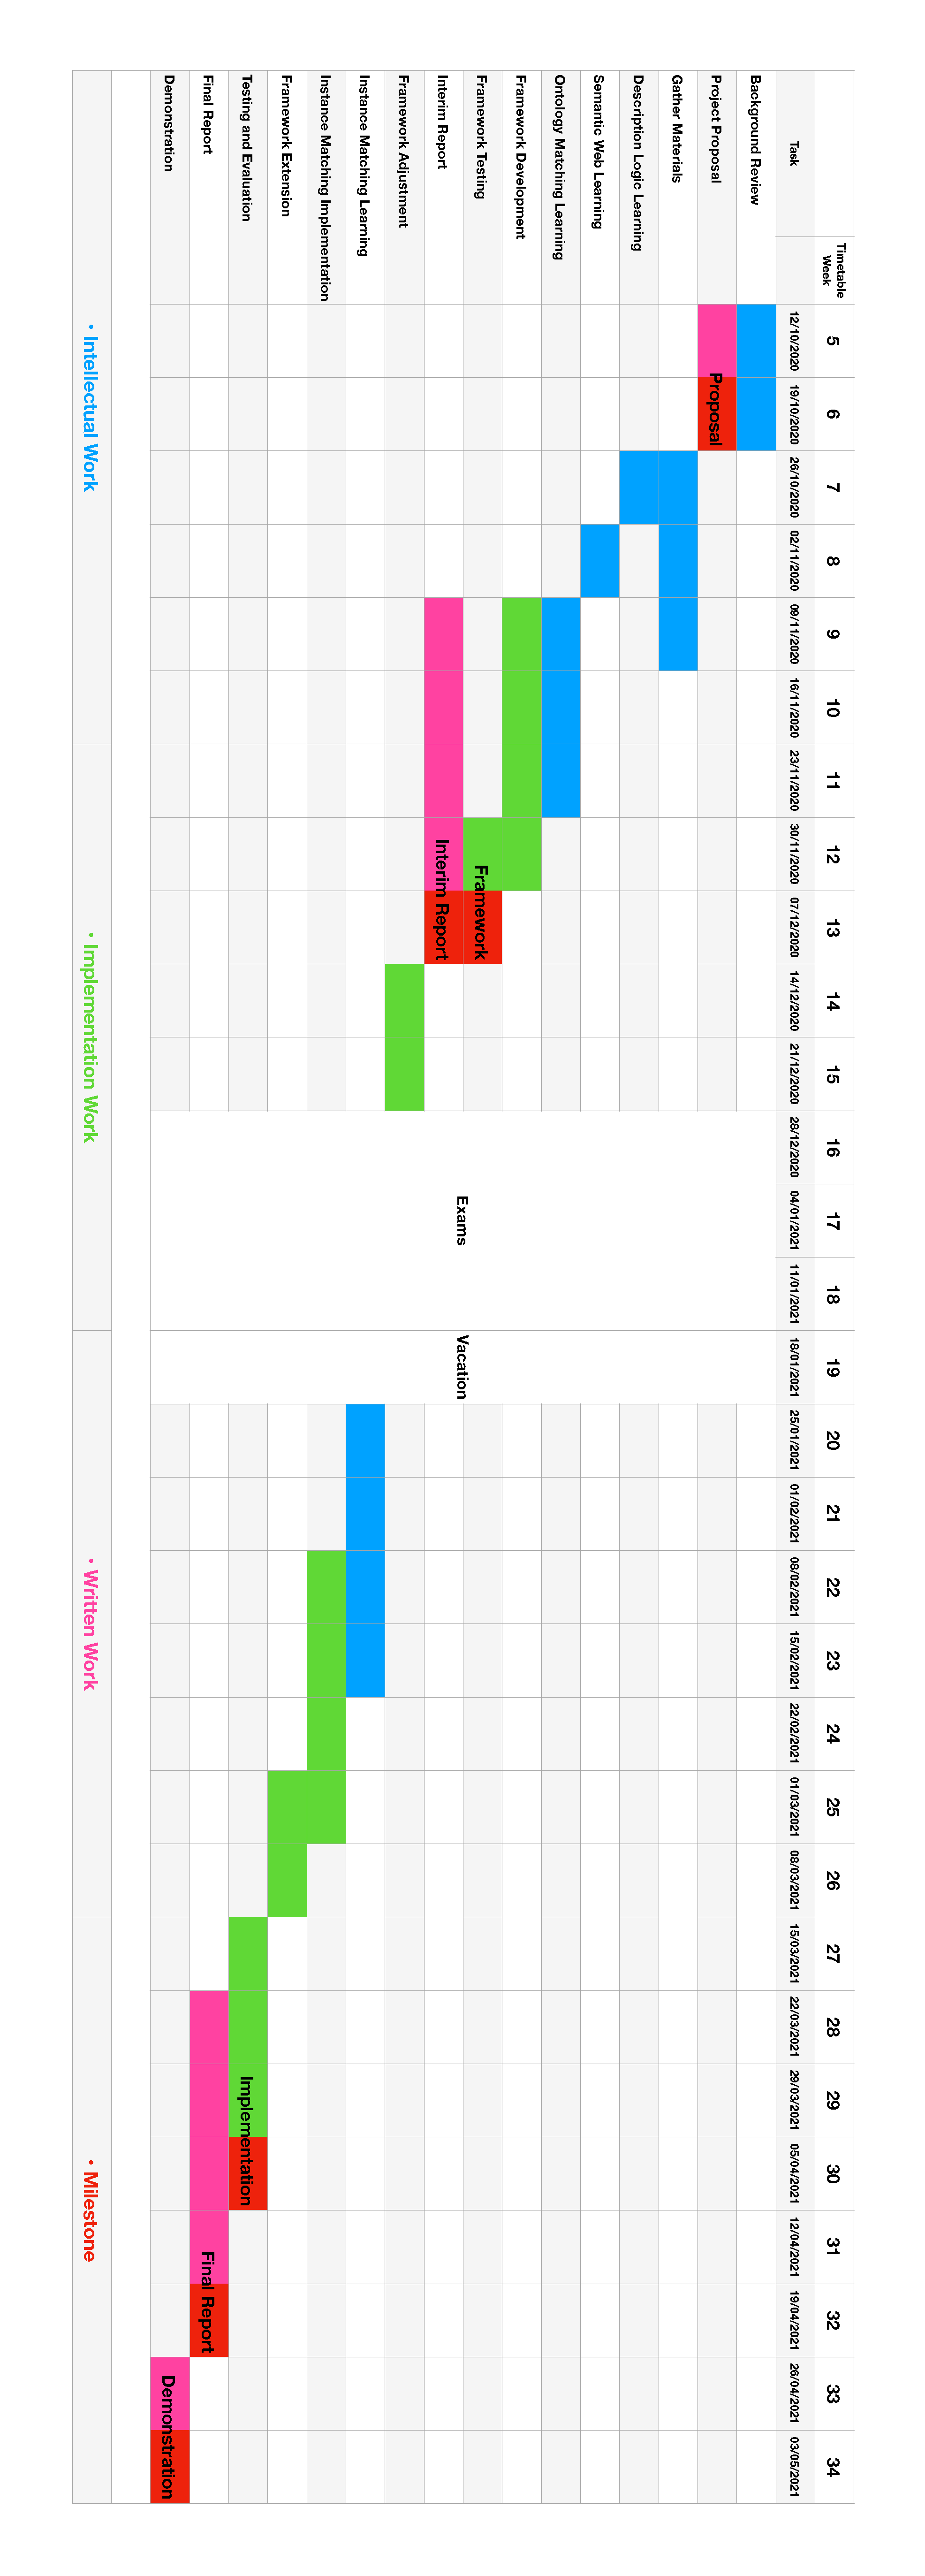
\includegraphics[width=\textwidth]{img/Gantt_old.pdf}
\caption{Original workplan}
\label{fig:Gantt_old}
\end{subfigure}
\begin{subfigure}[ht]{0.5\textwidth}
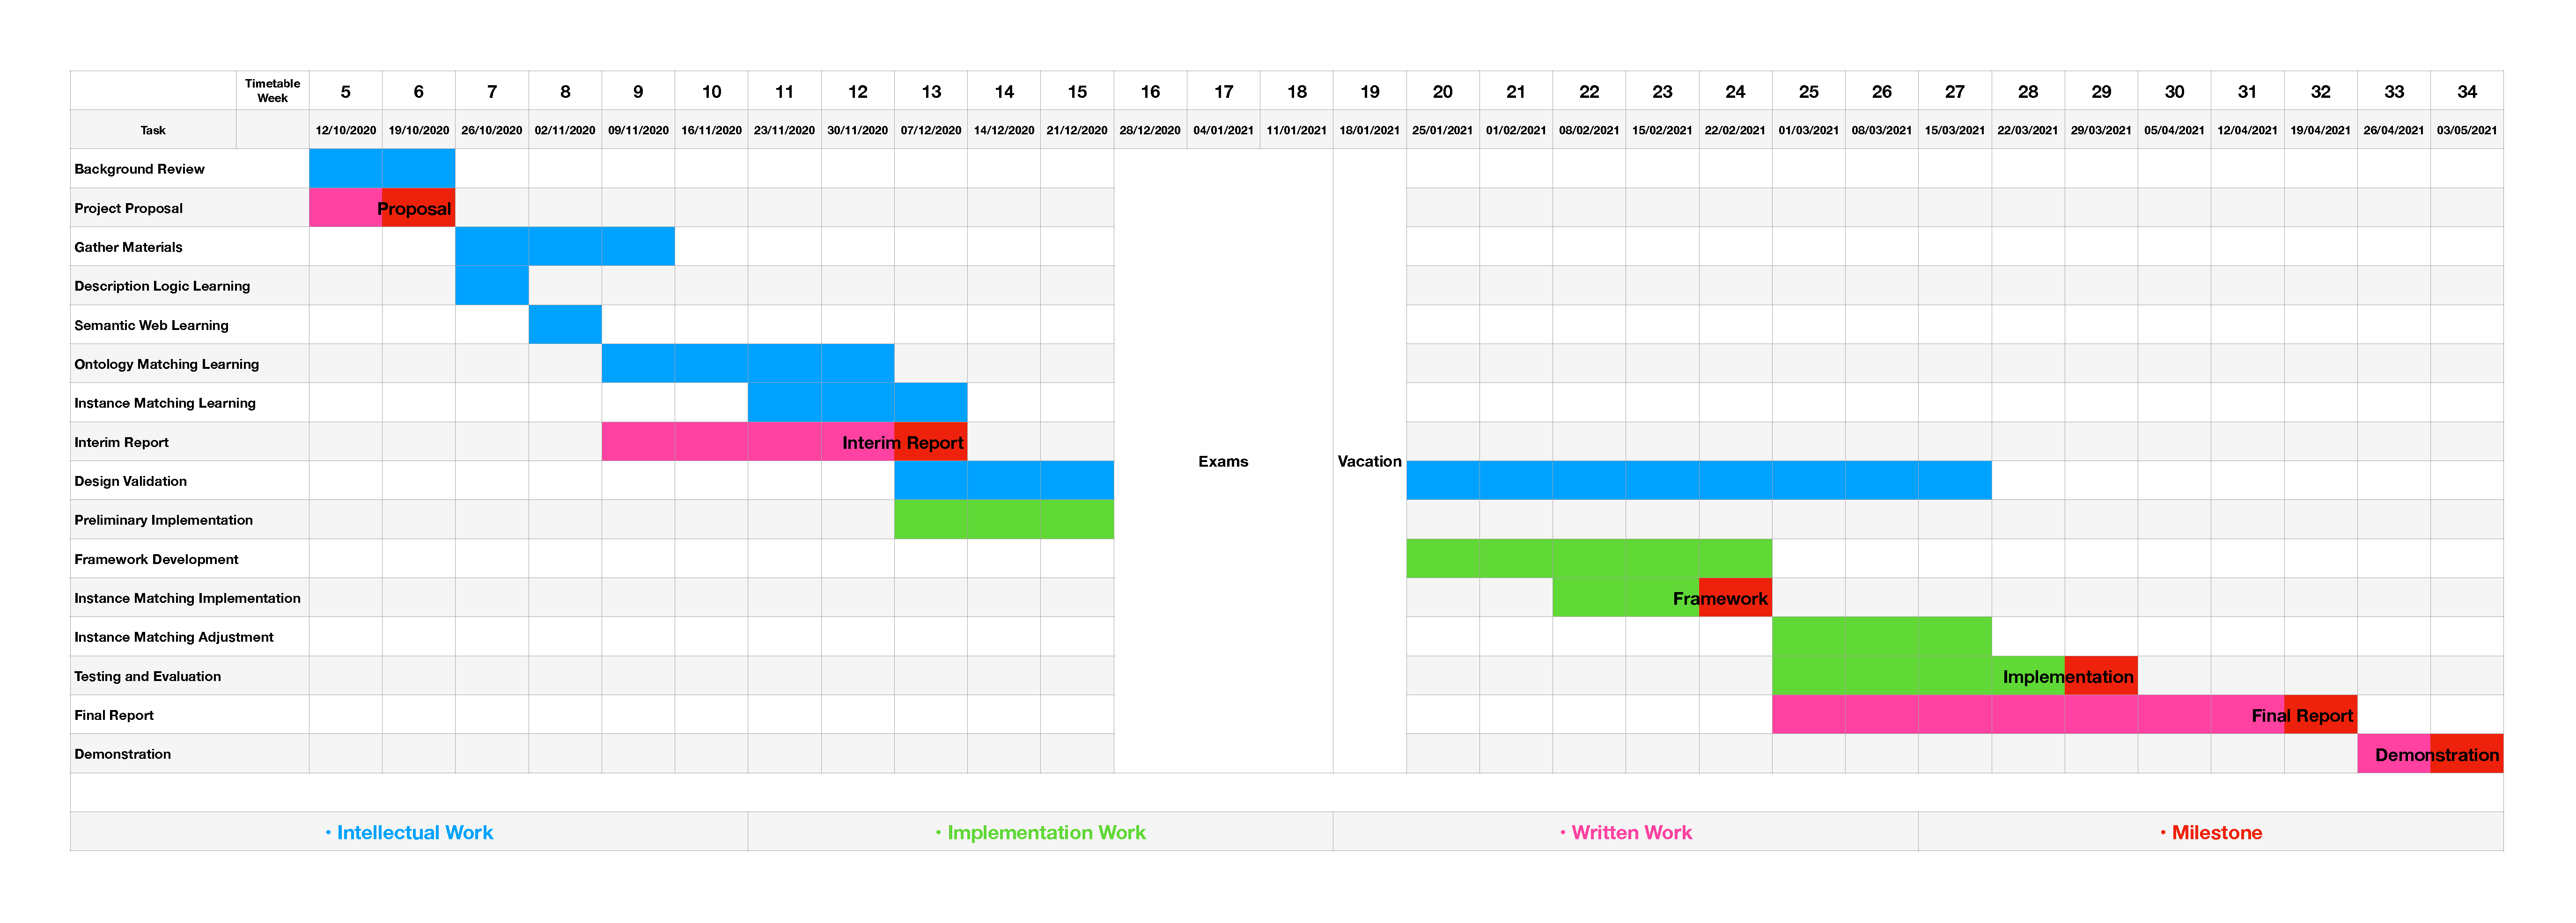
\includegraphics[width=\textwidth]{img/Gantt_new.pdf}
\caption{Revised workplan}
\label{fig:Gantt_new}
\end{subfigure}
\caption{Revision of workplan}
\label{fig:Gantt}
\end{figure}

\subsection{Working Methodology}
% Scrumban methodology.
While the workplan is designed with respect to the Waterfall methodology \cite{balaji2012waterfall} for clear validation of progress against the milestones, a hybrid combination of the Scrum and Kanban methodologies, namely Scrumban \cite{DBLP:conf/ispw/NikitinaKS12}, was adopted and followed as the working methodology since the beginning. The Scrum aspect splits the workload into small, easily achievable goals which could be reviewed regularly, while a Kanban board enables clear monitoring of the process, with tasks being assigned in dynamic ``lanes'' (see figure \ref{fig:Kanban}\footnote{\url{https://github.com/Jizhou-Che/Dissertation/}}). Fusing the two together exploits the advantages of both: the workflow can adapt to changes quickly, and since all tasks are visualised, the efforts can be well balanced and coordinated. The sprint interval for Scrumban was set to 1 week, which is the interval between every consecutive meetings with my supervisor. This helped tremendously in pushing everything forward, so that the project can progress at a good pace despite the intense curricular work and my lack of experience in carrying out a large project like this individually.

\begin{figure}[ht]
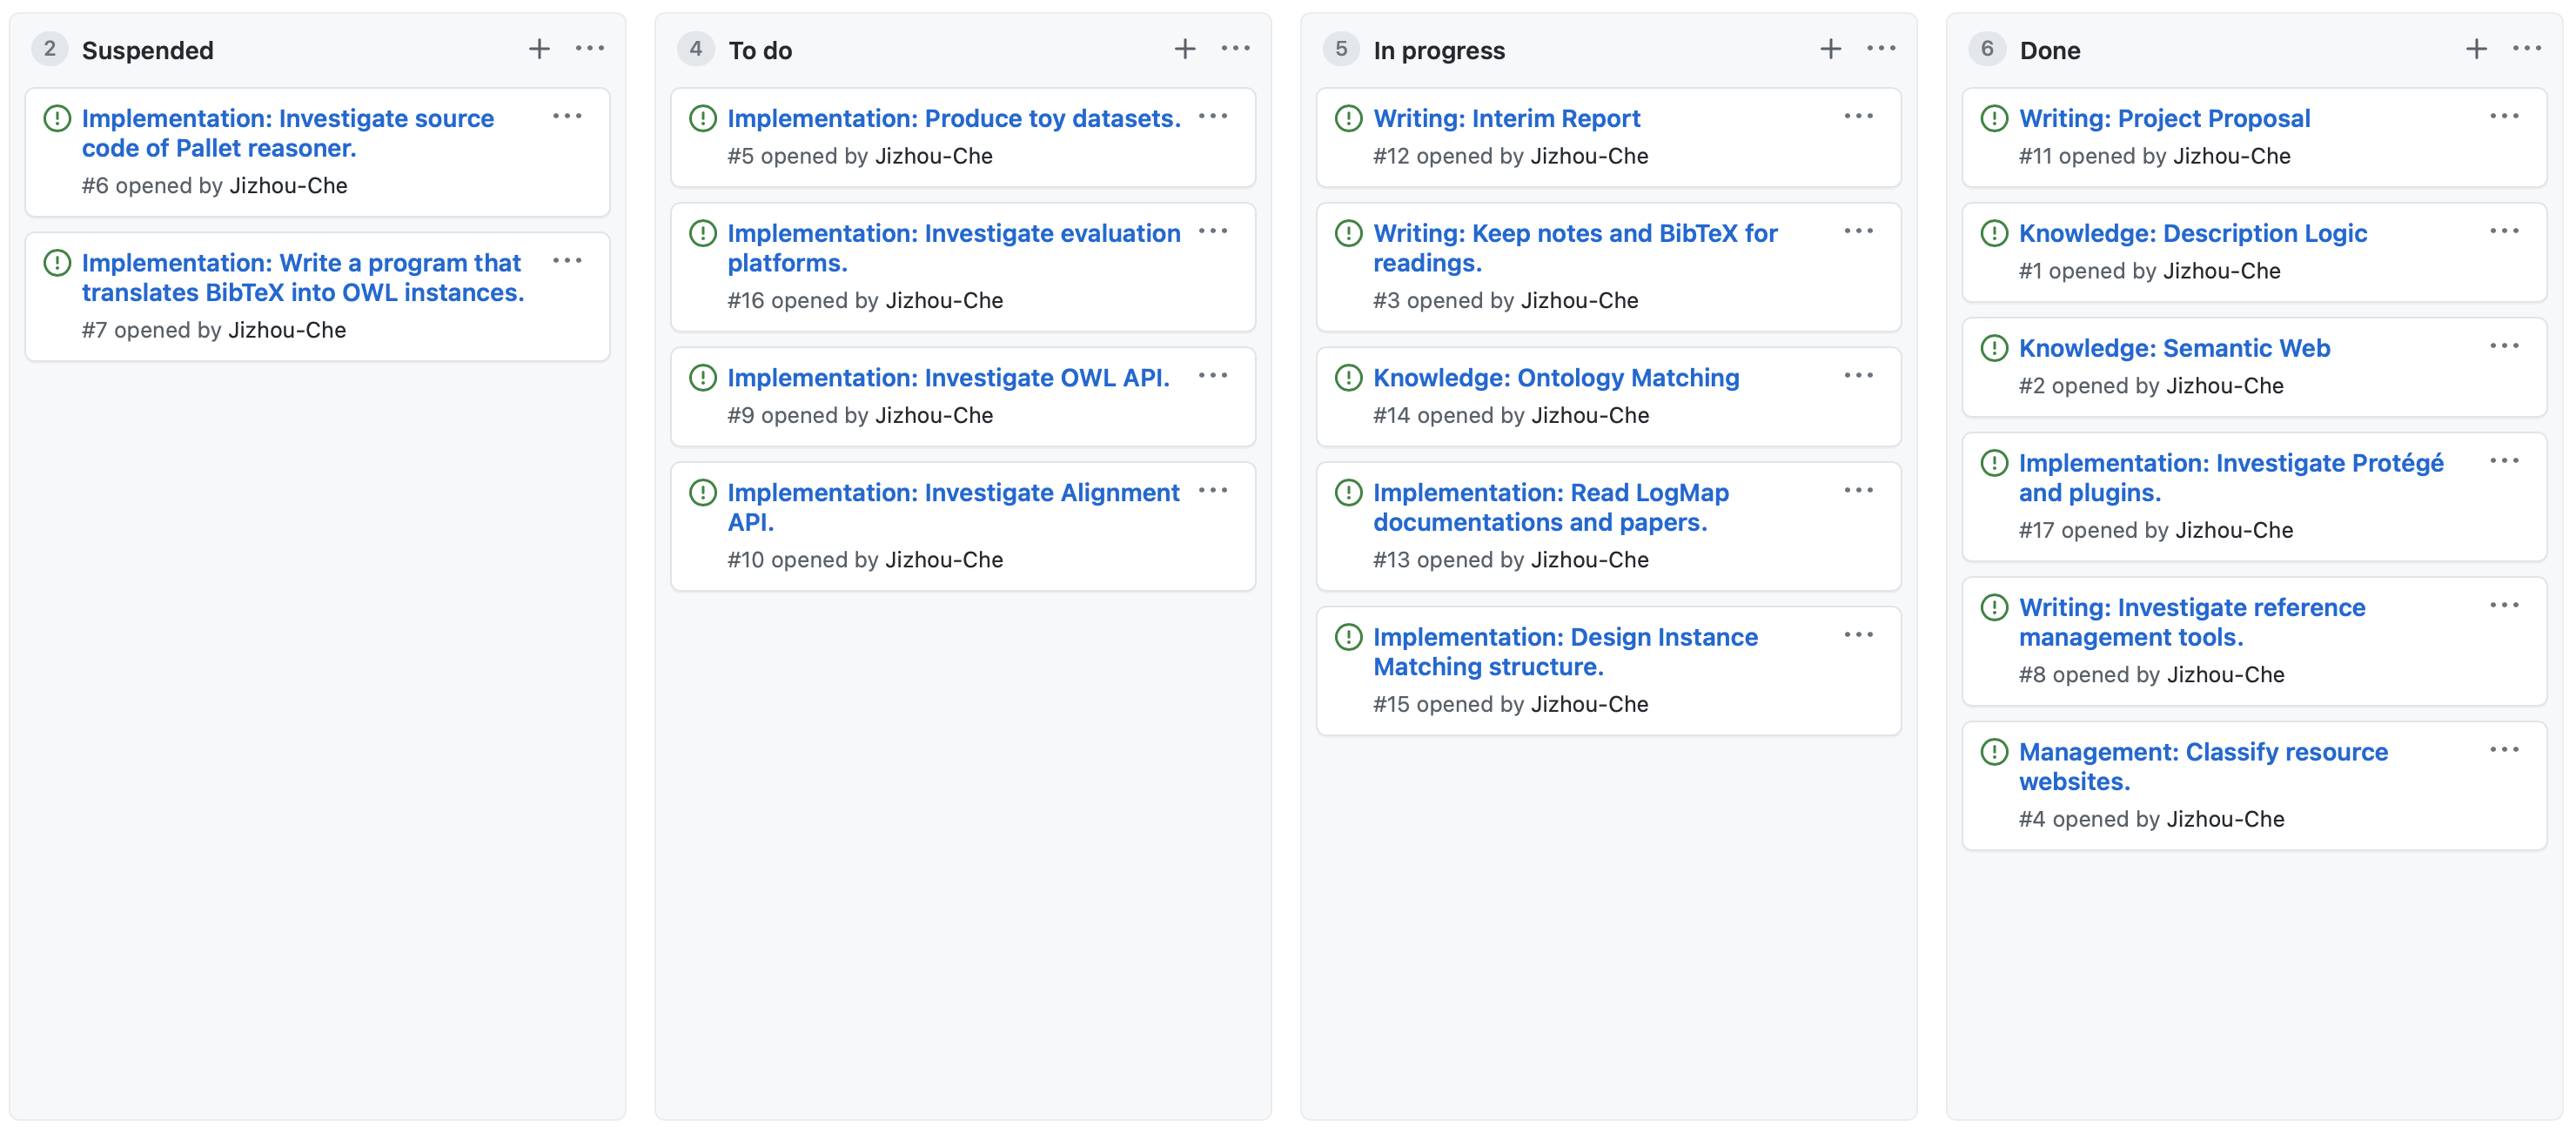
\includegraphics[width=\textwidth]{img/Kanban.png}
\caption{Kanban Board}
\label{fig:Kanban}
\end{figure}

\subsection{Resource Management}
% Resource management.
All resources related to the project, such as meeting minutes, reading notes and source code have been managed with the Git version control system and consistently pushed to GitHub. They can be found at \url{https://github.com/Jizhou-Che/Dissertation}. This has proven to be a good practice, in that the evolution of the project is documented within the accumulation and development of resources. The project have been adhering to this methodology throughout.

\subsection{Contingency Measures}
% Risks that may arise in the revised workplan, and how they can be mitigated and managed.
Admittedly, I did not put too much thought into contingency measures at the start of the project. However, I have learned its necessity though my experience in managing this long-term project. Based on the issues I have encountered in the first part of the project as well as my personal observations, the most significant risks that can arise in the process are pointed out below, as well as the proposed strategies to mitigate their effects.
\\\\
Underestimating the steepness of learning curves or the difficulty of implementation can disrupt the regular time allocation, and therefore shake the entire workplan. Apart from foreseeing the issue and allocate adequate amount of time in advance, time can be borrowed from flexible tasks that are less affected by a shrink of timespan. While this provides a temporary solution that mitigates the impact to the workplan, ultimately extra time should be dedicated to the project as compensation.
\\\\
The workloads of other modules is another serious issue, especially when their deadlines are close to the project milestones. This can not only disrupt the time management, but also increase the psychological pressure. Low moods and anxiety can lead to a drop in the productivity as well as the quality of work produced. Having tried the relax-then-focus approach, that was not suitable for me as the guilty only increased. Instead, trying to finish the work together with a friend has proved to be more effective.
\\\\
Offline meetings can sometimes be inappropriate due to wellbeing or other issues. In such cases online meetings via Zoom were organised, and have proven equal effectiveness.


\section{Reflections}
% A personal reflection on the plan and your experience of the project (a critical appraisal of how the project went).
I have faced challenges in various aspects of the project. Academically, the steep learning curve of background knowledge made the workload that was already intense even heavier, and the locating of quality resources for knowledge acquisition required professional judgment and guidance especially at the beginning. My supervisor helped me a lot in such aspects, so I could dive quickly into solid work. For example, after given a brief introduction to description logic as the foundation of OWL ontologies, I picked some books and online learning materials for self-study. My supervisor helped assessing the quality of my selections, and pointed out where I should investigate first to get started, which was extremely helpful to me. My supervisor also suggested excellent ideas when I needed to consider different approaches. For example, when producing an initial set of rules used for reasoning, my supervisor suggested adding assumptions such as disjoint siblings to the set. This has proved to increase the number of correct mappings produced especially for ontologies with poorly defined schema-level information. At times when I got stuck for lacking knowledge or data, my supervisor directed me to prestigious professors, papers and websites so I could acquire just the resources I needed. This equipped me with solid understanding about the core subjects I had been dealing with throughout the project. I also got a lot of help regarding academic writing from my supervisor, in the form of either oral instructions or written feedback. These served as a golden standard whenever I needed to draft something professional.
\\\\
Regarding the implementation steps, when exploring the prominent ontology matching systems at the beginning, it seemed intimidating that even a lite version of a matching system is constructed from so many components, with thousands of lines of code to investigate within each of them. Although being comfortable with Java programming, I did not know where to start for quite some time. It was after I have accumulated sufficient amount of knowledge by reading the relevant literatures and supporting documents that the meaning of code segments became clearer to me. Also, testing the entire system gives only the matching result, which did not contribute to the understanding of the programme itself. Therefore, I started by extracting individual modules and classes and tested them with intermediate results generated by debugging tools. This ultimately enabled me to build up a solid understanding of the logic and semantics of the programmes, so I could know where my own implementation should start with, as well as how some of the existing modules can be adapted to my implementation framework. My supervisor inspired me with implementation ideas as well. For example, when I got stuck at parsing the reference alignment from RDF to TXT format, my supervisor shared some existing code pieces with me, and by investigating them I discovered that it is possible to render all acceptable formats into an internal data structure, which simplified my implementation greatly.
\\\\
Considering project management, time allocation was the largest difficulty I encountered, as it was hard to balance the project with other curricular subjects, and sometimes my judgment of the amount of time required for a task was inadequate. Sometimes I feel like I could have used some of my time more wisely, for instance, investigating matching systems based on fuzzy logic did not really help with my implementation, but there was no telling that without having done the work. Therefore, I consider this as a necessary stage that must be gone through to toughen my skills and enrich my experience, and I feel I have made advancements in my time management abilities at the end of the project. Managing the resources is what I did best. By preparing for the meetings and keeping the minutes well-organised at all time, I hardly had any trouble locating any information that was previously discussed in the meetings. Academic resources such as books, research papers and evaluation websites were indexed separately so that they are always easy to access. My own writing and implementation have been managed using version control since the beginning, so I never suffered from lost of data under any circumstances.
\\\\
I feel truly fulfilled at the end of the project, having learned a lot of fundamental theories about logical reasoning and knowledge representation and processing. These are subjects I wished to learn before doing the project, and I am proud to be able to achieve my goals in the end. Apart from that, I find myself becoming a competent user of OWL ontology language, semantic web technology, the related tools, and of course, Java programming. These are solid skills that could not be acquired without practicing with them in a large project. Finally, I am no longer terrified by large projects development and management, as even the most complex project can be done though cumulative effort, which is exactly what I have done through this project. I will certainly benefit from all of these invaluable experience in my future academic works.
